% = = = = = = = = = = = = = = = = = = = = = = = = = = = = = = = = = = = = = = = = = = = = =
% P  R  E  A  M  B  L  E
% = = = = = = = = = = = = = = = = = = = = = = = = = = = = = = = = = = = = = = = = = = = = =
\documentclass[12pt]{article}
\usepackage{amsmath, amssymb, authblk}
%\usepackage{array}
\usepackage{booktabs}
\usepackage{bm}
\usepackage[small,labelfont=bf,up,singlelinecheck=false]{caption}
%\usepackage{fancyhdr}
%\usepackage[T1]{fontenc}
\usepackage[bottom]{footmisc}
\usepackage{geometry}
\usepackage{graphicx}
\usepackage{hyperref}
%\usepackage[utf8]{inputenc}
	%\inputencoding{latin1}
	%\inputencoding{utf8}
%\usepackage{lettrine}
%\usepackage[sc]{mathpazo}
%\usepackage{lmodern} % Nice fonts?
%\usepackage{mathrsfs}
\usepackage{mathtools} 
\usepackage{marvosym} % silly bullet-point symbols (misc symbols)
%\usepackage{microtype}
\usepackage{minitoc}         % left in case it is needed elsewhere
\setcounter{secttocdepth}{5} % idem
\usepackage{etoc} % for toc before each section.
%\usepackage{multicol}
\usepackage{Needspace}
\usepackage{paralist}
%\usepackage{polynom} 			% typesetting polynomial long division
%\usepackage{setspace}
%	\onehalfspacing 
\usepackage[compact]{titlesec} 		% compact shrinks whitespace around section headings.
% \usepackage{ulem} 				% for strikeout \sout command.
%\usepackage{verbatim}

% Muh packagez :)
%\usepackage{../Packages/ClassCommands}
\usepackage{../Packages/BrandonColors}
%\usepackage{../Packages/BrandonBoxes}
\usepackage{../Packages/NoteTaker}
%\usepackage{../Packages/MachineLearningUtils}

\newcommand\myfig[2][0.3\textwidth]{\begin{figure}[h!]\centering\includegraphics[width=#1]{#2}\end{figure}}
\newcommand{\myspace}{\vspace{2\bigskipamount}}
\newcommand\p{\Needspace{10\baselineskip} \noindent}


\titleformat*{\subsubsection}{\large\scshape}

% Title
\title{\vspace{-10mm}\fontsize{24pt}{8pt}\selectfont\textbf{Fall 2016 Course Notes}\vspace*{-4mm}}
% Author
\author{Brandon McKinzie}
% Date
\date{}

% --------------------------------------------------------------
% --------------------------------------------------------------


\begin{document}
\dosecttoc
%\tableofcontents



\mysection{Condensed Summaries}\label{Condensed Summaries}

\lecture{Condensed Summaries}{Conv Nets: A Modular Perspective}{December 21}


\p \href{https://colah.github.io/posts/2014-07-Conv-Nets-Modular/}{From this post on Colah's Blog}. 

\myspace The title is inspired by the following figure. Colah mentions how groups of neurons, like $A$, that appear in multiple places are sometimes called \textbf{modules}, and networks that use them are sometimes called modular neural networks. You can feed the output of one convolutional layer into another. With each layer, the network can detect higher-level, more abstract features.
\myfig[0.3\textwidth]{ColahConv2.PNG}
\begin{compactitem}[$\longrightarrow$]
	\item Function of the $A$ neurons: compute certain \textit{features}.
	
	 \item Max pooling layers: kind of ``zoom out''. They allow later convolutional layers to work on larger sections of the data. They also make us invariant to some very small transformations of the data.
\end{compactitem}



\lecture{Condensed Summaries}{Understanding Convolutions}{December 21}


\p \href{https://colah.github.io/posts/2014-07-Understanding-Convolutions/}{From Colah's Blog}. 

\p \blue{Ball-Dropping Example}. The posed problem:
\begin{footnotesize}
\begin{quote}
	Imagine we drop a ball from some height onto the ground, where it only has one dimension of motion. How likely is it that a ball will go a distance c if you drop it and then drop it again from above the point at which it landed?
\end{quote}
\end{footnotesize}

\begin{figure}[h!]
	\centering
	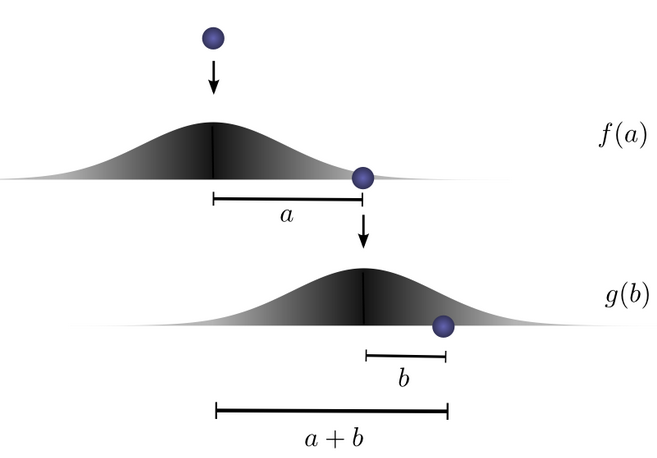
\includegraphics[width=0.35\textwidth]{ColahBall.PNG}
	\hspace{2cm}
	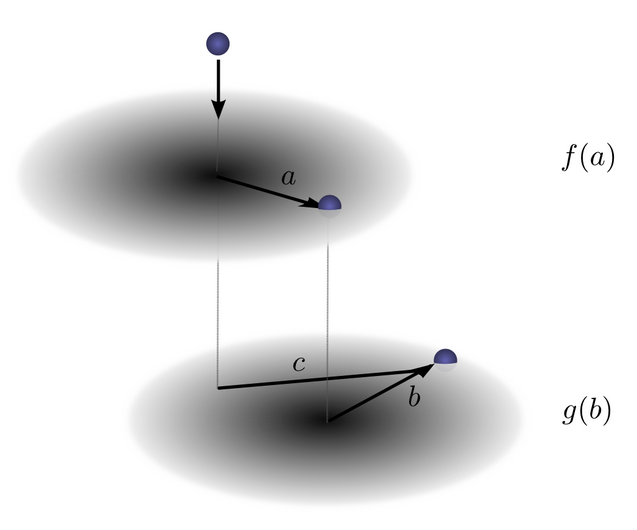
\includegraphics[height=0.25\textwidth]{ColahBall3.PNG}
\end{figure}

From basic probability, we know the result is a sum over possible outcomes, constrained by $a + b = c$. It turns out this is actually the definition of the convolution of $f$ and $g$. 
\begin{align}
	\mathrm{Pr(a + b = c)} &= \sum_{a + b = c} f(a) \cdot g(b) \\
	(f * g)(c) &= \sum_{a + b = c} f(a) \cdot g(b)\\
	&= \sum_a f(a) \cdot g(c - a)
\end{align}

\myspace
\p \blue{Visualizing Convolutions}. Keeping the same example in the back of our heads, consider a few interesting facts. 
\begin{itemize}
	\item \textbf{Flipping directions}. If $f(x)$ yields the probability of landing a distance $x$ away from where it was dropped, what about the probability that it was dropped a distance $x$ from where it \textit{landed}? Apparently\footnote{Not entirely sold on the generalization of this, or even how true it is here.} it is $f(-x)$. 
	
	\myfig[0.3\textwidth]{ColahBall2.PNG}
	
	\item Above is a visualization of one term in the summation of $(f * g)(c)$. It is meant to show how we can move the bottom around to think about evaluating the convolution for different $c$ values. 
\end{itemize}
We can relate these ideas to image recognition. Below are two common kernels used to convolve images with. 
\begin{figure}[h!]
	\centering
	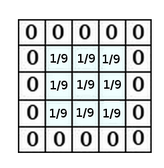
\includegraphics[width=0.15\textwidth]{ColahKernel1.PNG}
	\hspace{2.5cm}
	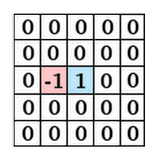
\includegraphics[height=0.15\textwidth]{ColahKernel2.PNG}
\end{figure}

On the left is a kernel for \textit{blurring} images, accomplished by taking simple averages. On the right is a kernel for \textit{edge detection}, accomplished by taking the difference between two pixels, which will be largest at edges, and essentially zero for similar pixels.


\lecture{Condensed Summaries}{Deep Reinforcement Learning}{December 23}

\href{https://www.nervanasys.com/demystifying-deep-reinforcement-learning/}{Link to tutorial} -- Part I of ``Demystifying deep reinforcement learning.'' \\


\p \blue{Reinforcement Learning}. Vulnerable to the \textit{credit assignment problem} - i.e. unsure which of the preceding actions was responsible for getting some reward and to what extent. Also need to address the famous \textit{explore-exploit dilemma} when deciding what strategies to use. 


\myspace
\p \blue{Markov Decision Process}. Most common method for representing a reinforcement problem. MDPs consist of states, actions, and rewards. Total reward is sum of current (includes previous) and \textit{discounted} future rewards:
\begin{equation}
	R_t = r_t \gamma(r_{t + 1}
	 + \gamma(r_{t + 2} + \ldots)) = r_t + \gamma R_{t + 1}
\end{equation}

\myspace
\p \blue{Q - learning}. Define function $Q(s, a)$ to be best possible score at end of game after performing action $a$ in state $s$; the ``quality'' of an action from a given state. The recursive definition of Q (for one transition) is given below in the \textit{Bellman equation}. 
$$ Q(s, a) = r + \gamma \max_{a'} Q(s', a') $$
and updates are computed with a learning rate $\alpha$ as
$$ Q(s_t, a_t) = (1 - \alpha)\cdot Q(s_{t -1}, a_{t - 1})
 + 	\alpha \cdot (r + \gamma \max_{a'} Q(s'_{t + 1}, a_{t+1}') ) $$
 
 \myspace
 \p \blue{Deep Q Network}. Deep learning can take deal with issues related to prohibitively large state spaces. The implementation chosen by DeepMind was to represent the Q-function with a neural network, with the states (pixels) as the input and Q-values as output, where the number of output neurons is the number of possible actions from the input state. We can optimize with simple squared loss:
 
 \myfig{DRL_loss.PNG}

and our algorithm from some state $s$ becomes
\begin{compactitem}
	\item[1.] \textbf{First forward pass} from $s$ to get all predicted Q-values for each possible action. Choose action corresponding to max output, leading to next $s'$.
	 
	\item[2.] \textbf{Second forward pass} from $s'$ and again compute $\max_{a'} Q(s', a')$. 
	
	\item[3.] \textbf{Set target output} for each action $a'$ from $s'$. For the action corresponding to max (from step 2) set its target as $r + \gamma \max_{a'} Q(s', a')$, and for all other actions set target to same as originally returned from step 1, making the error 0 for those outputs. (Interpret as update to our guess for the best Q-value, and keep the others the same.)
	
	\item[4.] \textbf{Update weights} using backprop. 
\end{compactitem}


\myspace
\p \blue{Experience Replay}. This the most important trick for helping convergence of Q-values when approximating with non-linear functions. During gameplay all the experience $<s, a, r, s'>$ are stored in a replay memory. When training the network, random minibatches from the replay memory are used instead of the most recent transition. 

\myspace
\p \blue{Exploration}. One could say that initializing the Q-values randomly and then picking the max is essentially a form of exploitation. However, this type of exploration is \textit{greedy}, which can be tamed/fixed with \textbf{$\bm{\varepsilon}$-greedy exploration}. This incorporates a degree of randomness when choosing next action at \textit{all} time-steps, determined by probability $\varepsilon$ that we choose the next action randomly. For example, DeepMind decreases $\varepsilon$ over time from 1 to 0.1. 

\myspace
\p \blue{Deep Q-Learning Algorithm}. 

% https://www.nervanasys.com/wp-content/uploads/2015/12/Screen-Shot-2015-12-21-at-11.23.43-AM-1.png
\myfig[0.75\textwidth]{DRL_alg.PNG}








\end{document}